\section{Datasets and Benchmarks}
\label{sec:datasets}

Cross-domain evaluation lives or dies by its data. Table~\ref{tab:survey-data} lists the dataset families most used in this literature, grouped by domain family, with the cross-domain caveats we consider decision-relevant.

\begin{table}[t]
\caption{Dataset families for cross-domain industrial anomaly detection. ``Cross-domain caveat'' records what limits each family's use in leave-one-domain-out evaluation.}
\label{tab:survey-data}
\centering
\small
\begin{tabular}{p{2.1cm}p{2.6cm}p{3.0cm}}
\toprule
Family & Representative data & Cross-domain caveat \\
\midrule
Semiconductor process & PHM16-CMP, SECOM, WM-811K & regression targets or batch tables; no fault labels; datasets are structurally heterogeneous (tabular vs.\ time series) \\
Rotating machinery & CWRU, Paderborn, MFPT, XJTU-SY, MaFaulDa & different rigs, fault taxonomies, and rates (12--128\,kHz); frequency-domain statistics vary strongly \\
Wind SCADA & CARE, EDP, Kelmarsh & heterogeneous feature counts; many releases unlabeled; status labels sparse/noisy \\
Solar PV & PVDAQ/OEDI, DKASC & mostly normal operation; anomalies often must be injected \\
Process/AIOps & SMD, SWaT, SMAP/MSL & different task semantics; not industrial machinery \\
Fleet/multi-factory & FactoryNet \cite{2605_09081} & new, promising; coverage still narrow \\
\bottomrule
\end{tabular}
\end{table}

Three observations shape how we treat benchmarks. First, \emph{fault taxonomy mismatch} is irreducible: a bearing inner-race fault, a fab removal-rate drift, and a wind turbine status code are not the same label space, so cross-industry transfer must be evaluated with unsupervised score-based metrics rather than shared classes. Second, \emph{label provenance is heterogeneous}: some datasets provide seeded faults (CWRU), some provide status codes (CARE), and others only a process target from which anomaly labels must be constructed (PHM16-CMP); any cross-domain claim inherits the weaknesses of the weakest protocol, and surveys of the field should demand explicit statements of how each label was produced. Third, several commonly used streams run to failure, which biases score statistics over time; temporal evaluation must account for degradation-ordered windows rather than assuming exchangeability \cite{2506_15831,2002_04236}.

We also note the field's data gap that matters most for employment-facing applications: no public \emph{mining-equipment SCADA} benchmark exists. Work that claims ``mining'' relevance currently substitutes rotating-machinery data (bearings, gearboxes) as the physically defensible proxy, and should say so explicitly. The recent emergence of large industrial corpora such as FactoryNet \cite{2605_09081} indicates movement, but process-industry coverage (fab, chemical, mining) remains thin, and foundation-model pretraining datasets rarely document ``industry family'' annotations, which limits their use in leave-one-industry-out protocols \cite{2502_03383,2510_26777}.

\section{Transfer Mechanisms}
\label{sec:transfer}

We organize cross-domain mechanisms into five families. The taxonomy is pragmatic: many methods combine families, and we use the primary mechanism as the grouping criterion (Figure~\ref{fig:taxonomy}).

\begin{figure}[t]
\centering
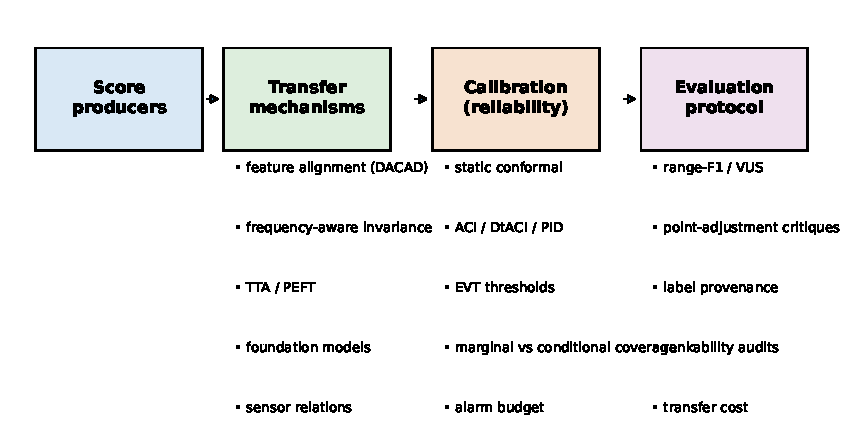
\includegraphics[width=\columnwidth]{fig_taxonomy.pdf}
\caption{Transfer mechanisms for cross-domain industrial anomaly detection, with representative citations per branch. Reliability (calibration) is deliberately drawn as a separate, orthogonal layer.}
\label{fig:taxonomy}
\end{figure}

\subsection{Feature Alignment and Discrepancy Minimization}
The mainstream approach learns representations whose source/target marginals match: adversarial alignment, maximum-mean-discrepancy variants with source weighting \cite{2310_14790}, contrastive objectives with anomaly injection \cite{dacad2024,2411_00914}, and source-free variants that adapt without source data \cite{2503_08749}. These methods produce competitive results on leave-one-condition-out benchmarks, but two failure modes recur across domains: alignment in feature space is frequency-agnostic, so it can erase band-specific fault signatures \cite{freqmatters2025}; and when the label spaces differ (anomaly-injection taxonomies do not transfer), contrastive gains shrink---in leave-one-industry-out settings, feature-space alignment has not consistently beaten plain reconstruction baselines \cite{2503_23060}.

\subsection{Frequency-Aware Invariance}
A newer branch makes spectral structure explicit: frequency-guidance losses for multi-source domain generalization in bearing diagnosis \cite{2502_00545}, band-level consistency objectives, and diagnostic studies that isolate spectral shift as a failure driver \cite{freqmatters2025,foundational2025}. The design question this branch confronts is preservation: aligning spectral statistics across domains can remove the very bands in which target faults live, motivating objectives that align domain-common bands while preserving saliency of fault-specific ones. In our own leave-one-industry-out benchmark \cite{our_scc}, such invariant objectives were neutral at attainable scales---an honest negative result that the branch must address with controlled shift gradients rather than null ablations.

\subsection{Test-Time Adaptation and Parameter-Efficient Adaptation}
TTA updates a small part of the model at deployment using unlabeled target data: low-rank input/output calibrators with frequency and robustness losses \cite{petsa2025}, normalization-statistic adaptation, concept-drift-aware online objectives \cite{2412_08435}, and TTA designed specifically for unsupervised time-series anomaly detection \cite{2312_11976}. Related streaming methods use regime detection to schedule adaptation \cite{2603_27814,2604_01845}. A recurring safety issue: in anomaly detection, adapting on the test stream can absorb the anomalies themselves into ``normal''---the adaptation objective must actively avoid explaining faults, not merely chase low reconstruction error \cite{2312_11976}.

\subsection{Foundation Models and Zero-Shot Transfer}
Time-series foundation models promise zero-shot transfer \cite{chronos2024}; critiques find their advantages narrow on shifted industrial series, where spectral coverage and domain diversity decide outcomes \cite{freqmatters2025,foundational2025,2502_03383,2510_26777}. Context-parroting baselines and simple forecasters remain tough to beat \cite{2505_11349}; industrial-specific foundations are emerging for bearings \cite{2504_01373} and as retrieval/agent systems \cite{2506_02081}. In our 6-fold benchmark \cite{our_scc}, a zero-shot foundation model (Chronos-bolt-small) transferred as a score producer but was matched or beaten by a 1.3M-parameter reconstruction encoder on five of six domain families---evidence that \emph{transfer mechanism} and \emph{model size} should be evaluated orthogonally.

\subsection{Sensor-Relation and Graph Structure}
Physical coupling among sensors is a transferable structural prior: graph anomaly detection formalisms \cite{2302_00058,2307_03759}, adaptive segmentation with structural features for rotating machinery \cite{2504_20756}, and relation-consistency objectives that penalize divergence of cross-channel dependency structure between domains. These methods are attractive when channel sets overlap; under disjoint sensor sets the relation structure must be constructed from physical roles rather than learned names, and relation alignment reduces to designing an equivariant channel embedding---an open design problem.
